\section{Methoden und Tools}

Zur Erstellung des Klassifikators nutzten wir, wie \citet{esteva2017dermatologist}, auch das öffentlich zur Verfügung stehende GoogleNet Inception v3, welches ein \textit{convolutional neural network} ist und aus zahlreichen verschiedenen Schichten und Neuronen besteht \citep{szegedy2016rethinking}. Dieses neuronale Netz wurde auf den Bildern des \textit{ImageNet} vortrainiert \citep{russakovsky2015imagenet}. Die von uns genutzten Gewichte stammen aus der Tensorflow (\cite{tensorflow2015-whitepaper}) Bibliothek ``slim''.
Ein solches vorheriges Training auf ImageNet etabliert einige grundlegende Strukturen im neuronalen Netz. Es werden Merkmalsdetektoren gelernt, die anschließend in dem Training der eigentlichen Aufgabe verfeinert werden.  Das Training und die damit verbundene Vorverarbeitung implementierten wir mittels \textit{Python}, in Kombination mit \textit{Tensorflow} (\cite{tensorflow2015-whitepaper}), \textit{Scikit-Learn} (\cite{scikit-learn}) und \textit{NumPy}. Für die Evaluierung wurde außerdem noch Matlab verwendet.

Als Datensatz nutzten wir die ISIC-Datenbank (\cite{ISIC}), welche aus insgesamt 13.768 Bildern von sowohl malignen als auch benignen Hautläsionen besteht. Von den Datensätzen, die von \citet{esteva2017dermatologist} genutzt wurden, ist dieser der Einzige, welcher frei verfügbar ist. Die Bilder dieses Datensatzes sind durch eine pathologische Untersuchung gelabelt worden. Somit sind die vorhandenen Daten relativ zuverlässig. Wir teilten den Datensatz drei Teildatensätze auf: einen Trainingsdatensatz, einen Validierungsdatensatz sowie einen Testdatensatz. Dabei beträgt der Anteil der Trainingsdaten $60\%$ und die Anteile der Validierungs- sowie der Testdaten jeweils $20\%$ aller Bilder. Diese wurden zufällig den Datensätzen zugeordnet.

Es stellte sich heraus, dass die Verteilung der Bilder dieses Datensatzes auf die verschiedenen Klassen (maligne/benigne) sehr unausgeglichen ist. Der Anteil der malignen Läsionen ist viel geringer als der Anteil der benignen Läsionen. Dieses Problem gingen wir durch eine spezielle Art der Randomisierung an. Während des Trainings trennten wir die Menge der Trainingsbilder in die Klassen \textit{maligne} und \textit{benigne} auf. Anschließend haben wir die Minibatches\todo{Puh das ist schon ein krasses Wort in nem deutschen report :D}, welche in das Netz gegeben wurden, aus Bildern dieser beiden Klassen zufällig befüllt. Dabei war die Wahrscheinlichkeit, dass ein Bild aus der Klasse der malignen Bilder stammt $p=0.5$. Somit wurde dieser unausgeglichene Datensatz ausbalanciert.

Ein weiteres Problem des ISIC-Datensatzes war die variable Größe der einzelnen Bilder. Für ein problemloses Trainieren des Netzes haben wir die Bilder daher vorverarbeitet. Dazu wurden die Bilder auf die kleinste verfügbare Größe skaliert. Für das Training des Netzes verwendeten wir, analog zu \citet{esteva2017dermatologist}, das maximale zentrale Quadrat des Bildes und skalierten es auf $299$px$\times 299$px herunter. Somit hatten wir eine homogene Menge an Bildern, die wir nun in einen Trainings-, Validierungs- und einen Testdatensatz unterteilten.

Während des Trainings wurden die Bilder zufällig augmentiert. Durch eine Augmentierung wird der Datensatz künstlich vergrößert um mehr diverse Trainingsbeispiele für das neuronale Netz zu erhalten. Dazu wendet man eine klassenerhaltende Transformation auf das Bild an. In unserem Ansatz setzen wir viele verschiedene Augmentierungen, die jeweils zufällig auf ein Bild angewendet wurden, ein. Abbildung~\ref{fig:aug} zeigt diese Augmentierungen anhand einer Beispielläsion.

\begin{figure}[t]
	\centering
	\begin{subfigure}[t]{0.24\linewidth}
		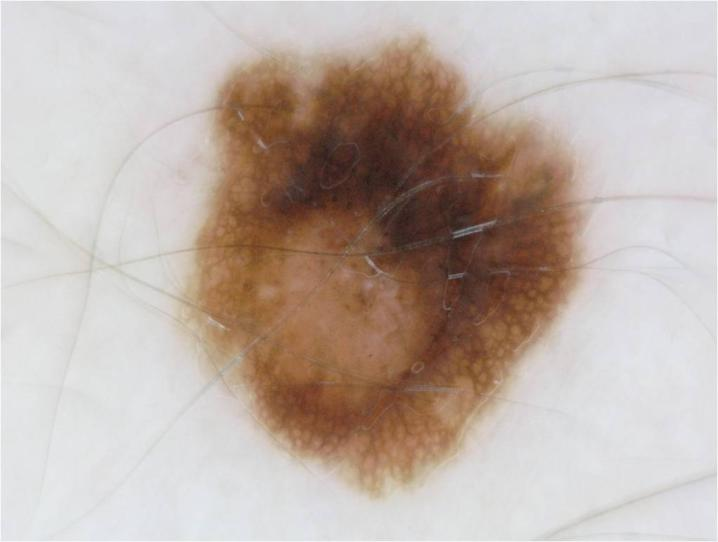
\includegraphics[width=\textwidth]{pics/augmentations/original.jpg}
		\caption{Original}
		\label{subfig:aug_original}
	\end{subfigure}
	\begin{subfigure}[t]{0.24\linewidth}
		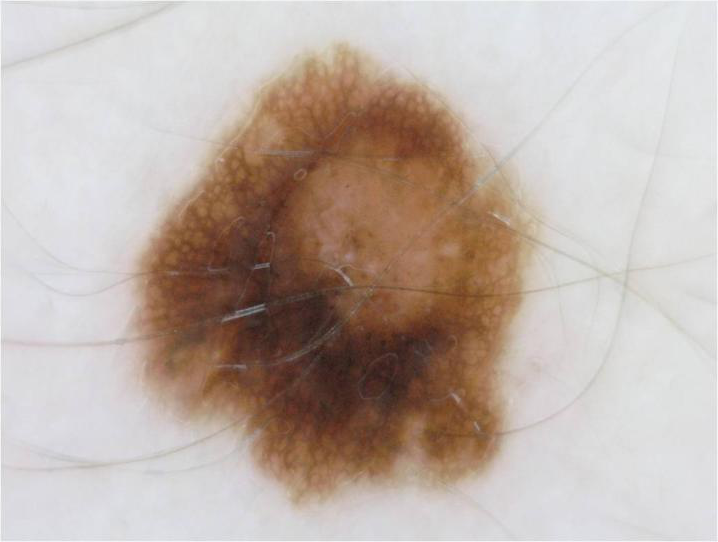
\includegraphics[width=\textwidth]{pics/augmentations/rotation.png}
		\caption{Rotation}
		\label{subfig:aug_rot}
	\end{subfigure}
	\begin{subfigure}[t]{0.24\linewidth}
		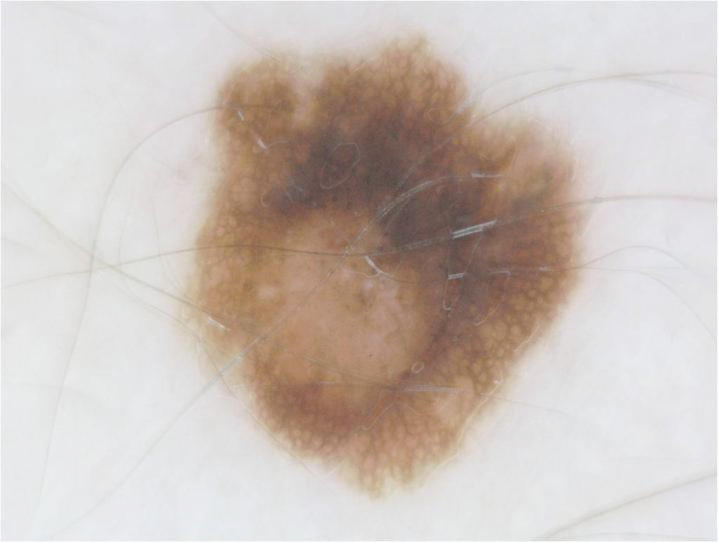
\includegraphics[width=\textwidth]{pics/augmentations/brightness.png}
		\caption{Helligkeit}
		\label{subfig:aug_bright}
	\end{subfigure}
	\begin{subfigure}[t]{0.24\linewidth}
		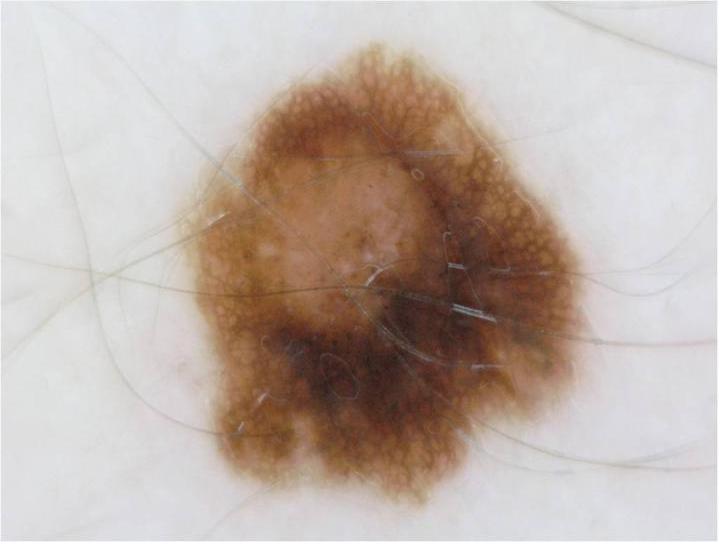
\includegraphics[width=\textwidth]{pics/augmentations/vertical_flip.png}
		\caption{Vertikale Spiegelung}
		\label{subfig:aug_v_flip}
	\end{subfigure}
	\begin{subfigure}[t]{0.24\linewidth}
		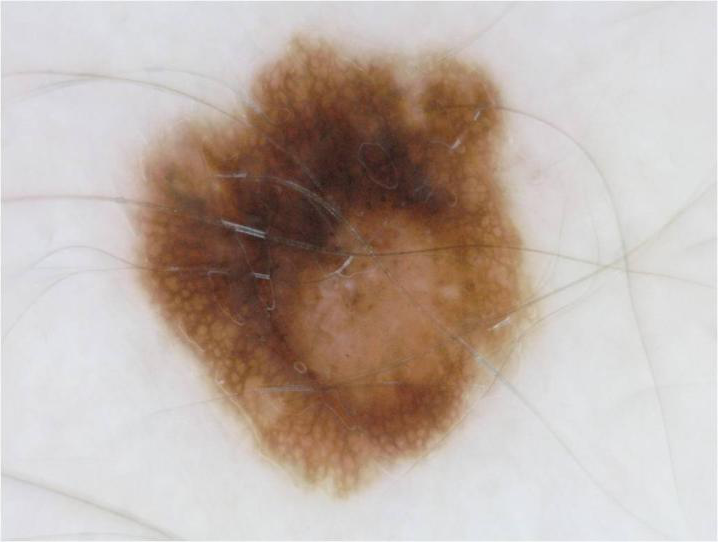
\includegraphics[width=\textwidth]{pics/augmentations/horizontal_flip.png}
		\caption{Horizontale Spiegelung}
		\label{subfig:aug_h_flip}
	\end{subfigure}
	\begin{subfigure}[t]{0.24\linewidth}
		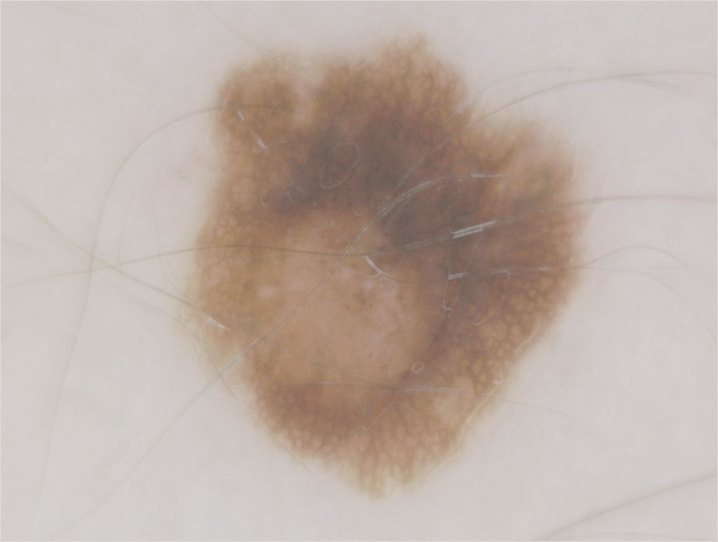
\includegraphics[width=\textwidth]{pics/augmentations/contrast.png}
		\caption{Kontrast}
		\label{subfig:aug_contrast}
	\end{subfigure}
	\begin{subfigure}[t]{0.24\linewidth}
		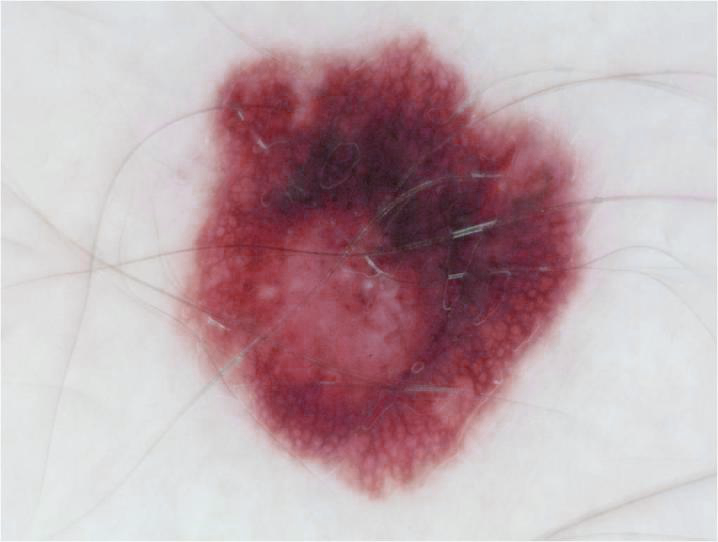
\includegraphics[width=\textwidth]{pics/augmentations/hue.png}
		\caption{Farbwert (Hue)}
		\label{subfig:aug_hue}
	\end{subfigure}
	\begin{subfigure}[t]{0.24\linewidth}
		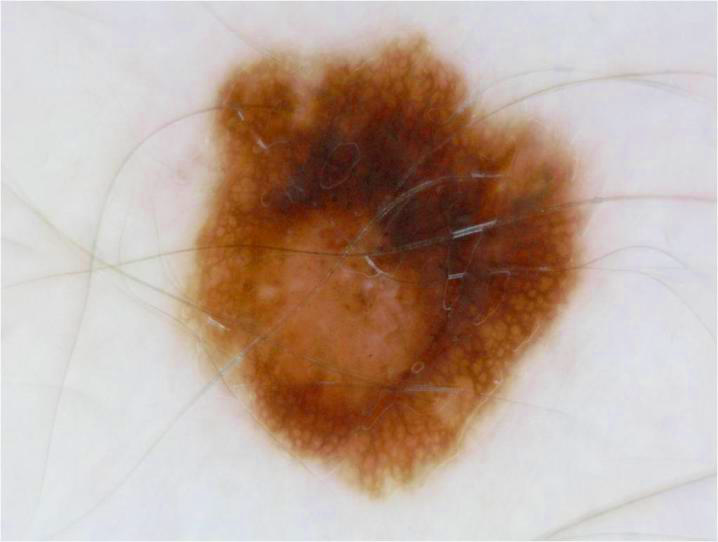
\includegraphics[width=\textwidth]{pics/augmentations/saturation.png}
		\caption{Sättigung}
		\label{subfig:aug_sat}
	\end{subfigure}
	\caption{Augmentierungsmethoden angewendet auf das originale Bild (\ref{subfig:aug_original})}
    \label{fig:aug}
\end{figure}


\begin{enumerate}
    \item \textbf{Rotation} (Abbildung \ref{subfig:aug_rot}): Bei dieser Transformation werden die Bilder je um 0$^{\circ}$, 90$^{\circ}$, 180$^{\circ}$ oder 270$^{\circ}$ gedreht. Diese Augmentierung soll das Netz invariant gegenüber Rotation machen. Dies ist wichtig, da die Orientierung der aufgenommenen Bilder willkürlich ist.
    
    \item \textbf{Helligkeit} (Abbildung \ref{subfig:aug_bright}):  Die Helligkeit der Bilder wird hier um einen zufälligen Wert erhöht oder verringert. So soll dem Netz eine gewisse Invarianz gegenüber verschiedenen Lichtbedingungen antrainiert werden.
    
    \item \textbf{Vertikales Spiegeln} (Abbildung \ref{subfig:aug_v_flip}): Bei dieser Methode werden die Bilder vertikal gespiegelt. Hierbei wird die Charakteristik der Läsion nicht verändert, jedoch werden so weitere Trainingsbilder erzeugt. 
    
    \item \textbf{Horizontales Spiegeln} (Abbildung \ref{subfig:aug_h_flip}):  In diesem Fall werden die Bilder horizontal gespiegelt. Auch hier wird die Charakteristik der Läsion nicht verändert, lediglich weitere Trainingsbilder erzeugt.
    
    \item \textbf{Kontrast} (Abbildung \ref{subfig:aug_contrast}):  Analog zur Helligkeit wird hier der Kontrast um einen zufälligen Wert erhöht oder erniedrigt. Auch dies soll das Netz invariant gegenüber wechselnden Lichtverhältnissen machen und zudem die Trainings-Menge vergrößern.
    
    \item \textbf{Farbwert (Hue)} (Abbildung \ref{subfig:aug_hue}):  Hier wird der Farbwert der Bilder zufällig verändert. Durch diese Methode soll die Unterscheidung der Klassen robuster gegenüber Farbänderungen in den Bildern gemacht werden.
    \todo{erwähnen, dass bei Hautärzten hauptsächlich die Form und nicht die Farbe der Läsionen eine Rolle spielt} 
    
    \item \textbf{Sättigung} (Abbildung \ref{subfig:aug_sat}):  Die Sättigung der Bilder wird zufällig um einen gewissen Wert verändert. Auch dies soll gegen abweichende Lichtverhältnisse helfen und die Menge der Trainingsdaten vergrößern.
\end{enumerate}

\subsection{Training}
\label{training}

	Das Training des GoogLeNet Inception v3 (\cite{inception}) implementierten wir in Tensorflow (\cite{tensorflow2015-whitepaper}). Dem Netz wurden Minibatches \todo{minibatch...} von jeweils sechs Bildern gezeigt. Von den augmentierten und zugeschnittenen Bildern wurde vor dem Forward-Pass \todo{Kurz erklären} der Mittelwert der Bilder des ImageNet Datensatzes (\cite{russakovsky2015imagenet}) abgezogen. Dies ist ein gängiger Vorgang, um die Verteilung der RGB-Werte und die Verteilung der RGB-Werte des ImageNet Datensatzes anzupassen. Nach einem Forward-Pass berechneten wir einen Loss. Auf diesem Loss trainierten wir das neuronale Netz mit dem \textit{Adam-Optimizer} und einer Lernrate $\eta=0.000001$. Im Folgenden Abschnitt werden die getesteten Loss-Funktionen näher erläutert.
	
\subsubsection{L1-Loss}

	Dieser Loss berechnet die absolute Abweichung der Vorhersage von den wahren Labels:
	\begin{align*}
		L = \sum_{i = 0}^C \mid lab_i - x_i\mid
	\end{align*}
	Dabei ist $C$ die Anzahl der Klassen, $lab$ die wahren Label und $x$ die Vorhersage des neuronalen Netzes.
	
	Das Ziel eines Trainings mit diesem Loss ist es, möglichst viele Nullen in dem Ergebnis-Vektor zu erhalten, da der L1-Loss spärliche (sparse) Lösungen begünstigt.

\subsubsection{L2-Loss}
	Dieser Loss berechnet die quadratische Abweichung der Vorhersage von den wahren Labels:
	\begin{align*}
	L = \sum_{i = 0}^C ( lab_i - x_i)^2
	\end{align*}
	Dabei ist $C$ die Anzahl der Klassen, $lab$ die wahren Label und $x$ die Vorhersage des neuronalen Netzes.
	
	Das Ziel eines Trainings mit diesem Loss ist es, große Fehler stark zu bestrafen und die Abweichungen von den wahren Labels so klein wie möglich, jedoch nicht zwingend $=0$, zu halten.
	
\subsubsection{Softmax-Kreuzentropie-Loss}
	Dieser Loss nutzt das Maß der Kreuzentropie, um den Loss zu berechnen. Dabei wird zunächst die Softmax-Funktion auf die Vorhersage und die Label angewendet und anschließend die Kreuzentropie der beiden Verteilungen berechnet.
	
	Dieser Loss wird dazu benutzt, um Verteilungen einander anzupassen. In unserem Ansatz verwendeten wir jedoch einen Vektor der Länge zwei als Klassenlabel. Bei solch einer kleinen Anzahl an Werten erwarteten wir, dass diese Loss-Funktion vergleichsweise schlecht abschneidet.
		
Um die oben angesprochene Unausgeglichenheit der Klassen in unserem Datensatz weiter zu balancieren und um eine bessere Performance für maligne Läsionen zu erreichen, nutzten wir bei dem L1-, wie auch bei dem L2-Loss zusätzlich einen Gewichtsterm. Dieser gewichtete die Abweichungen abhängig von der Zielklasse. Dabei wurden die Werte mit $lab=$ maligne mit $3$ und die Werte mit $lab=$ benigne mit $0.5$ multipliziert. 
	  

\subsection{Analysemethoden}
\label{analysemethoden}

Für die Bewertung und Optimierung unseres Klassifizierers wurden verschiedene Methoden angewandt. Die Genauigkeit konnte mit unserem Datensatz nur unter großer Skepsis betrachtet werden. Sie berechnet sich durch die Anzahl der richtig vorhergesagten Stichproben dividiert durch die Anzahl aller Stichproben:
	\[\text{Accuracy} = \frac{TP+TN}{TP+TN+FP+FN}\]
Da der in diesem Projekt verwendete Datensatz deutlich mehr negative als positive Beispiele enthält, können unter dieser Berechnung sehr hohe Genauigkeiten auftreten, obwohl eventuell kein positives Beispiel richtig berechnet wurde.
Eine weitaus bessere Analyse ist möglich, indem die richtig positiven und richtig negativen Beispiele getrennt betrachtet werden. Die Sensitivität, auch richtig-positiv-Rate oder auch Recall genannt, entspricht in unserem Fall dem Anteil an tatsächlich malignen Hautläsionen, bei denen diese auch als maligne erkannt wurde:
\[\text{Sensitivität} = \frac{TP}{TP+FN}\]
Die Spezifität, auch richtig-negativ-Rate genannt, entspricht dem Anteil an tatsächlich benignen Hautläsionen, die auch als benigne erkannt wurden:
\[\text{Spezifität} = \frac{TN}{TN+FP}\]
Die getrennte Betrachtung beider Werte erlaubt es uns direkt zu sehen, ob maligne oder benigne Beispiele besser erkannt werden und dementsprechend zu optimieren.

Zusätzlich zogen wir noch den \textit{Matthews correlation coefficient} in Betracht. Dieser wird als Qualitätsmaßstab in binären maschinellen Lernmethoden verwendet, im Speziellen wenn der Datensatz sehr unausgeglichen ist. 

\[\text{MCC} = \frac{TP*TN - FP*FN}{\sqrt{(TP+FP)*(TP+FN)*(TN+FP)*(TN+FN)}}\]

Im Gegensatz zu den anderen hier verwendeten Methoden, liefert der MCC Werte zwischen $-1$ und $1$. Ein MCC von $0$ ist somit nicht besser als eine Zufallsvorhersage. Ein MCC von $1$ hingegen steht für eine komplette Übereinstimmung, während $-1$ für die komplette Missklassifizierung steht.

Außerdem verwendeten wir noch den F2-Score als Qualitätsmaßstab. Der F1-Score ist das harmonische Mittel zwischen dem Recall und der Precision, der F2-Score dagegen gewichtet den Recall stärker und setzt somit den Schwerpunkt mehr auf die falsch negativen Stichproben, also die malignen Hautläsionen, die als benigne erkannt wurden:
	\[\text{Precision} = \frac{TP}{TP+FP}\]
    \[\text{Recall/Sensitivität} = \frac{TP}{TP+FN}\]
	\[\text{F1-Score} = 2*\frac{\text{precision}*\text{recall}}	{\text{precision}+\text{recall}}\]
   	\[\text{F2-Score} = 5*\frac{\text{precision}*\text{recall}}	{4*\text{precision}+\text{recall}}\]
    
Schließlich entschieden wir uns noch dazu, die Receiver-Operating-Characteristics-Kurve (ROC) und die dazugehörige \textit{area under the curve (AUC)} zu verwenden. Diese Methode stellt visuell die Abhängigkeit der Sensitivität von der falsch-positiv-Rate dar. Eine ROC-Kurve nahe der Diagonalen deutet auf eine Zufallsvorhersage hin und hat eine AUC von $0.5$. Eine gute ROC-Kurve liegt deshalb oberhalb der Diagonalen und steigt senkrecht an bevor die falsch-positiv-Rate erhöht wird. Eine AUC von $1$ steht somit für eine perfekte Klassifizierung, eine AUC von $0$ für komplette Missklassifizierung. In diesem Falle könnten die Labels einfach umgedreht werden. Ziel ist es also eine ROC-Kurve weit entfernt von der Diagonalen zu erhalten.
    
Wir entschieden uns bewusst für eine größere Anzahl von Qualitätsmaßstäben. Da ein Parameter für sich nie die Komplexität des Klassifizierers komplett beschreiben kann, sollen die verschiedenen Qualitätsmaßstäbe bei der Evaluierung und der Entscheidung für den für uns geeignetsten Klassifizierer als Gesamtheit betrachtet und verwendet werden. Dies ermöglicht es uns, die Klassifizierung gezielt in die von uns gewünschte Richtung zu lenken, um beispielsweise falsch negative Vorhersagen zu minimieren.

\subsection{Framework}

Um sowohl das Training als auch die Evaluation auf verschiedenen Systemen durchführen und Parameteränderungen leicht über die Konsole testen zu können, entwickelten wir ein Framework. Über dieses Framework können Trainingsdurchläufe einfach gestartet und später automatisiert evaluiert werden. Dabei lassen sich die Trainingsparameter (Batchsize, Loss-Funktion, Lernrate, Datensatz), sowie plattformspezifische Einstellungen, wie der Speicherort der Daten und den Bezeichner der gewünschten Grafikkarte, anpassen. Startet man das Python-Skript ``start\_training.py'' mit den entsprechenden Parametern, wird automatisch ein neuronales Netz geladen und trainiert, sowie die Log-Dateien und die Gewichte entsprechend gespeichert. Für die Evaluation können analog die Systemparameter sowie der Datensatz, auf dem das Netzwerk evaluiert werden soll, eingestellt werden (Validierungsdatensatz oder Testdatensatz).


